\documentclass[letterpaper]{article}
\usepackage[T1]{fontenc}
\usepackage[utf8]{inputenc}
\usepackage{tocloft,siunitx,amssymb,amsmath,graphicx}
\usepackage[top=3cm,left=3cm,right=3cm]{geometry}
\usepackage{float,pgf,pgfplots}
\usepackage[american]{circuitikz}
\graphicspath{{img/}}
\renewcommand\cftsecfont{\normalfont}
\renewcommand\cftsecpagefont{\normalfont}
\renewcommand{\cftsecleader}{\cftdotfill{\cftsecdotsep}}
\renewcommand\cftsecdotsep{\cftdot}
\renewcommand\cftsubsecdotsep{\cftdot}
\renewcommand\cftsubsubsecdotsep{\cftdot}
\title{Lab :}
\author{
    Sebastián Nava López\\
    \and
    Ericka Sabrina Pensamiento R.\\
    \and
    Salvador Palos Gil
}
%\captionsetup[subfigure]{justification=raggedright}
\begin{document}
\begin{titlepage}
    \centering
    {\Huge Instituto Politécnico Nacional}\\[3ex]
    {\huge Escuela Superior de Cómputo}\\[8ex]
    {\huge Fundamental Circuit Analysis}\\[12ex]
    {\Large Lab 5: Mesh Analysis}\\[20ex]
    {\Large Group: 1CV5 Team: 7 \\[8ex]
    Sebastian Nava López\\[4ex]
    Sabrina Erika Pensamiento Robledo\\[4ex]
    Salvador Palos Gil\\[18ex]
    }
    \large{Elaboration:April 17,2018 \hspace{8em} Due date:April 24,2018}
\end{titlepage}
\tableofcontents
\newpage
\section{Introduction}
\newpage
\section{Development}
\subsection{Verification of mesh analysis in DC}
Using a circuit as the one shown in fig: 
\begin{figure}[H]
    \centering
\begin{circuitikz}
    \draw
        (0,2) to [V](0,0)
        (0,2) -- (0,4)
        (0,4) to [R=$\SI{680}{\ohm}(R_1)$](3,4)
        to [V](6,4) to
        (6,2) to [R,*-](3,2)
        to [R,*-*](0,2)
        (6,2) to [R=$\SI{1}{\kilo\ohm}(R_5)$](6,0) -- (0,0)
        (3,0) to [R=$\SI{470}{\ohm}(R_4)$,*-](3,2)
        {
            [anchor = south east](5.4,2.2) node {$\SI{560}{\ohm}(R_3)$}
            [anchor = south east](2.4,2.2) node {$\SI{1}{\kilo\ohm}(R_2)$}
            [anchor = south east](0,1.4) node {$\SI{9}{\volt}(V_{S1})$}
            [anchor = south east](5.4,4.4) node {$\SI{5}{\volt}(V_{S2})$}
        }
        ;
\end{circuitikz}
\end{figure}
we measured current in each mesh ,and voltage values in each resistance.
\subsubsection{Calculations}
Using mesh analysis to calculate currents, we assign the direction of all currents clockwise, as
shown:
\begin{figure}[H]
    \centering
    \begin{circuitikz}
        \draw
        (0,2) to [V](0,0)
        (0,2) -- (0,4)
        (0,4) to [R=$R_1$](3,4)
        to [short,i_=$I_1$](3.5,4)
        to [V](6,4) to
        (6,2) to [R,*-](3,2)
        to [R,*-*](0,2)
        (6,2) to [R=$R_5$](6,0) -- (0,0)
        (3,0) to [R=$R_4$,*-](3,2)
        (3,0) to [short,i_=$I_2$](0,0)
        (6,0) to [short,i_=$I_3$](3,0)
        {
            [anchor = south east](5.4,2.2) node {$R_3$}
            [anchor = south east](2.4,2.2) node {$R_2$}
            [anchor = south east](0,1.4) node {$V_{S1}$}
            [anchor = south east](5.4,4.4) node {$V_{S2}$}
            [anchor = south east](1.8,0.7) node {$(2)$}
            [anchor = south east](4.9,0.7) node {$(3)$}
            [anchor = south east](3.4,2.7) node {$(1)$}
        }
        ;
    \end{circuitikz}
\end{figure}
Aplying Kirchhoff's Current Law(KCL) in mesh 1:
\begin{gather*}
    V_{R3}+V_{R2}+V_{R1}+V_{S2} = 0\\
    560(I_1-I_3)+1000(I_1-I_2)+680I_1+5 = 0
\end{gather*}\\[-7.5ex]
\begin{equation}2240I_1-1000I_2-560I_3 = -5\label{eq:1}\end{equation}
    in mesh 2:
\begin{gather*}
    -V_{S1}+V_{R2}+V_{R4} = 0\\
    -9+1000(I_2-I_1)+470(I_2-I_3) = 0
\end{gather*}\\[-7.5ex]
\begin{equation}-1000I_1+1470I_2-470I_3 = 5\label{eq:2}\end{equation}
    in mesh 3:
\begin{gather*}
    V_{R4}+V_{R3}+V_{R5} = 0\\
    470(I_3-I_2)+560(I_3-I_1)+100I_3 = 0
\end{gather*}\\[-7.5ex]
\begin{equation}-560I_1-470I_2-2030I_3 = 0\label{eq:3}\end{equation}
    therefore we have the following linear equation system:
    \[
        \begin{bmatrix}
            2240 & -1000 & -1560\\
            -1000 & 1470 & -470\\
            -560 & -470 & 2030
        \end{bmatrix}
    \begin{bmatrix}
        -5\\
        9\\
        0
    \end{bmatrix}
    =
    \begin{bmatrix}
        I_1\\
        I_2\\
        I_3
    \end{bmatrix}
\]
To solve the system using Crammer's rule we need to compute the required determinants($\Delta$). For
$\Delta$ we have that:
    \begin{gather*}
        \Delta = det\Bigg(
        \begin{bmatrix}
            2240 & -1000 & -560\\
            -1000 & 1470 & -470\\
            -560 & -470 & 2030
        \end{bmatrix}
        \Bigg)\\
        \Delta = 2240\cdot det\bigg(
        \begin{bmatrix}
            1470 & -470\\
            -470 & 2030
        \end{bmatrix}
        \bigg)
        +1000\cdot det\bigg(
        \begin{bmatrix}
            -1000 & -470\\
            -560 & 2030
        \end{bmatrix}
        \bigg)
        -560\cdot det\bigg(
        \begin{bmatrix}
            -1000 & 1470\\
            -560 & -470
        \end{bmatrix}
        \bigg)\\
        \Delta = 2240\cdot(2763200)+1000\cdot(-2293200)-560\cdot(1293200)\\
        \therefore\Delta = 3172200000
    \end{gather*}
$\Delta_1$ is given by:
    \begin{gather*}
        \Delta_1 = det\Bigg(
        \begin{bmatrix}
            -5 & -1000 & -560\\
            9 & 1470 & -470\\
            0 & -470 & 2030
        \end{bmatrix}
        \Bigg)\\
        \Delta_1 = -5\cdot det\bigg(
        \begin{bmatrix}
            1470 & -470\\
            -470 & 2030
        \end{bmatrix}
        \bigg)
        +1000\cdot det\bigg(
        \begin{bmatrix}
            9 & -470\\
            0 & 2030
        \end{bmatrix}
        \bigg)
        -560\cdot det\bigg(
        \begin{bmatrix}
            9 & 1470\\
            0 & -470
        \end{bmatrix}
        \bigg)\\
        \Delta_1 = -5\cdot(2763200)+1000\cdot(18270)-560\cdot(-4230)\\
        \therefore\Delta_1 = 6822800
    \end{gather*}
$\Delta_2$ is given by:
    \begin{gather*}
        \Delta_2 = det\Bigg(
        \begin{bmatrix}
            2240 & -5 & -560\\
            -1000 & 9 & -470\\
            -560 & 0 & 2030
        \end{bmatrix}
        \Bigg)\\
        \Delta_2 = 2240\cdot det\bigg(
        \begin{bmatrix}
            9 & -470\\
            0 & 2030
        \end{bmatrix}
        \bigg)
        +5\cdot det\bigg(
        \begin{bmatrix}
            -1000 & -470\\
            -560 & 2030
        \end{bmatrix}
        \bigg)
        -560\cdot det\bigg(
        \begin{bmatrix}
            -1000 & 9\\
            -560 & 0
        \end{bmatrix}
        \bigg)\\
        \Delta_2 = 2240\cdot(18270)+5\cdot(-2293200)-560\cdot(5040)\\
        \therefore\Delta_2 = 26636400
    \end{gather*}
$\Delta_3$ is given by:
    \begin{gather*}
        \Delta_3 = det\Bigg(
        \begin{bmatrix}
            2240 & -1000 & -5\\
            -1000 & 1470 & 9\\
            -560 & -470 & 0
        \end{bmatrix}
        \Bigg)\\
        \Delta_3 = 2240\cdot det\bigg(
        \begin{bmatrix}
            1470 & 9\\
            -470 & 0 
        \end{bmatrix}
        \bigg)
        +1000\cdot det\bigg(
        \begin{bmatrix}
            -1000 & 9\\
            -560 & 0
        \end{bmatrix}
        \bigg)
        -5\cdot det\bigg(
        \begin{bmatrix}
            -1000 & 1470\\
            -560 & -470
        \end{bmatrix}
        \bigg)\\
        \Delta_3 = 2240\cdot(4230)+1000\cdot(5040)-5\cdot(1293200)\\
        \therefore\Delta_3 = 16281200
    \end{gather*}
Finally:
\begin{gather*}
I_1 = \frac{\Delta_1}{\Delta} = \frac{6822800}{3172200000}\qquad\therefore I_1 =
\SI{2.151}{\milli\ampere}\\
I_2 = \frac{\Delta_2}{\Delta} = \frac{26636400}{3172200000}\qquad\therefore I_2 =
\SI{8.397}{\milli\ampere}\\
I_3 = \frac{\Delta_3}{\Delta} = \frac{8049200}{3172200000}\qquad\therefore I_3 =
\SI{2.537}{\milli\ampere}\\
\end{gather*}
Now that we have values for all the currents, voltage values in each resistor are given as follows:
Voltage in $R_1$:
\begin{gather*}V_{R1} = R_1\cdot I_1
    =(\SI{680}{\ohm})(\SI{2.151}{\milli\ampere})\\\therefore V_{R1} =
\SI{1.463}{\volt}
\end{gather*}
Voltage in $R_2$:
\begin{gather*}V_{R2} = R_2\cdot(I_2-I_1)
    =(\SI{1}{\kilo\ohm})(\SI{8.397}{\milli\ampere}-\SI{2.151}{\milli\ampere})\\\therefore V_{R2} =
\SI{6.246}{\volt}
\end{gather*}
Voltage in $R_3$:
\begin{gather*}V_{R3} = R_3\cdot(I_3-I_1)
    =(\SI{560}{\ohm})(\SI{2.537}{\milli\ampere}-\SI{2.151}{\milli\ampere})\\\therefore V_{R3} =
\SI{0.216}{\volt}
\end{gather*}
Voltage in $R_4$:
\begin{gather*}V_{R4} = R_4\cdot(I_2-I_3)
    =(\SI{470}{\ohm})(\SI{8.397}{\milli\ampere}-\SI{2.537}{\milli\ampere})\\\therefore V_{R4} =
\SI{2.754}{\volt}
\end{gather*}
Voltage in $R_5$:
\begin{gather*}V_{R5} = R_5\cdot I_3
    =(\SI{1}{\kilo\ohm})(\SI{2.537}{\milli\ampere})\\\therefore V_{R5} =
\SI{2.537}{\volt}
\end{gather*}
\subsubsection{Simulation}
\begin{figure}[H]
    \centering
    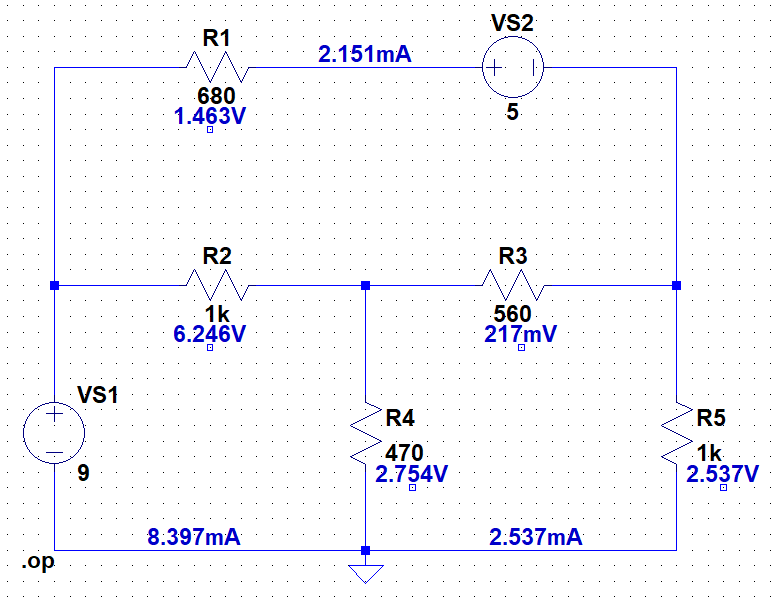
\includegraphics[width=.8\linewidth]{sim1}
    \caption{Circuit simulation}
\end{figure}
\subsubsection{Measurements}
\begin{figure}[H]
    \centering
    \begin{tabular}{|c|c|c|c|}\hline
        Measurements & Theoretical Value(\si{\milli\ampere}) & Measured Value(\si{\milli\ampere}) &
        Simulated Value (\si{\milli\ampere})\\\hline
        $I_{1}$ & 2.151 & 2.180 & 2.151 \\\hline
        $I_{2}$ & 8.397 & 8.460 & 8.397 \\\hline
        $I_{3}$ & 2.537 & 2.580 & 2.537 \\\hline
        $V_{R1}$ & 1.463 & 1.482 & 1.463 \\\hline 
        $V_{R2}$ & 6.246 & 6.250 & 6.246 \\\hline 
        $V_{R3}$ & 0.216 & 0.218 & 0.217 \\\hline 
        $V_{R4}$ & 2.754 & 2.783 & 2.754 \\\hline 
        $V_{R5}$ & 2.537 & 2.560 & 2.537 \\\hline 
    \end{tabular}
    \caption{Values from the mesh currents measured, calculated and simulated}
\end{figure}
\section{Questions}
\textit{\textbf{Explain the operation of the oscilloscope}}\\
%ans
\textit{\textbf{What's the function of the signal generator?}}\\
%ans
\textit{\textbf{What are the Lissajous graphs for?}}\\
%ans
\textit{\textbf{What are the operating modes Y (t) and XY used for?}}\\
%ans
\textit{\textbf{Which means by coupling in D.C.?}}\\
%ans
\textit{\textbf{What is an offset signal?}}\\
%ans
\textit{\textbf{Which means that a signal is out of phase?}}\\
%ans
\section{Conclusions}
{\large Sabrina:}\\
%
\\[2ex]
{\large Salvador:}\\
%
\\[2ex]
{\large Sebastián:}\\
%texto
\end{document}
